\chapter{Theory}

\subsection{Reservoir computing}


	\subsubsection{Formalities}

\begin{tabular}{c|c}
	\hline
	\textbf{U}& uniformly distribution \\
	\hline
	$u^{-h}=(u_{-h},u_{-h+1},u_{0}) \in \textbf{U}^h$ & sequence of numbers drawn from a uniform distribution  \\	
	\hline
	$\textbf{O}$ & set of Targets or \emph{true} values \\
	\hline
	$\hat{\textbf{O}}$ & set of Predictions that the system makes\\
	\hline
\end{tabular}

A reservoir computer needs to exhibit three properties in order to perform computations in a meaningful i.e. useful way.

\begin{itemize}
	\item echo state property - the system state is only an echo of all previous inputs fed into the system
	\item similar inputs create similar outputs
	\item
\end{itemize}


We can measure how well a dynamical system performs computations by testing it in a variety of benchmarks. Dynamical systems are continuously evolving in time, thus reservoir computation performance is usually tested on time-structured data. Benchmarks try to quantify the capacity to remember information previously fed into it and its ability to make nonlinear transformation of the data.\\ 

The used benchmarks have an input sequence $\textbf{U}(t)$ and a $target$ sequence $\textbf{O}(t)$ with $t \in \mathbb{Z}$ being the time counted in clockcycles (cc). For a specific time $t$ the reservoir offers a number of outputs $\textbf{x}_{k}(t)$ which can be linearily combined in order to reach some $predicted$ value $\hat{\textbf{O}}(t)$. Ideally $\hat{\textbf{O}}(t) = \textbf{O}(t)$ which would represent a perfect reconstruction of the target value through the system. Usually machine learning systems give imperfect predictions $\hat{\textbf{O}}(t)$ that vary from the \emph{true} value $\textbf{O}(t)$.

\subsubsection{Linear Memory Recall}
The simplest task a reservoir can perform is to simply repeat the the information that was fed into it at a certain point in time. 

	\begin{equation}
		\begin{split}
		O_{1}(t) & = u_{t - 1} \\
		O_{2}(t) & = u_{t - 2} \\				
		O_{3}(t) & = u_{t - 3} \\
				 &\;\; \vdots \\
		O_{n}(t) & = u_{t - n}
		\end{split}
		\label{eq:linear_recall_task}
	\end{equation}


\begin{figure}
	\centering
	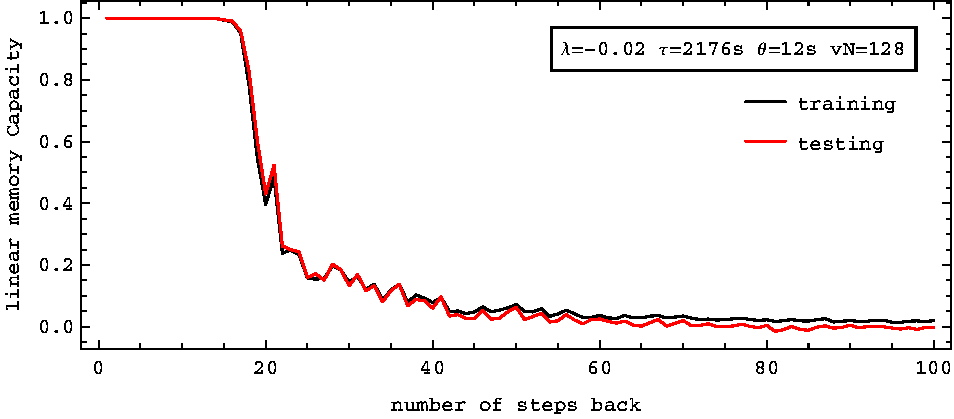
\includegraphics[width=0.99\linewidth]{pics/linearMemoryCurveN1}
	\caption{The linear memory capacities for varying steps into the past. The system is able to perfectly reproduce inputs up until $12$ steps into the past. $N=1, vN=128, \lambda=-0.02, \omega=1, \gamma=-0.1, \theta=12, \tau=2176$. }
	\label{fig:linearMemoryRecallCurveN1}
\end{figure}

\begin{figure}
	\centering
	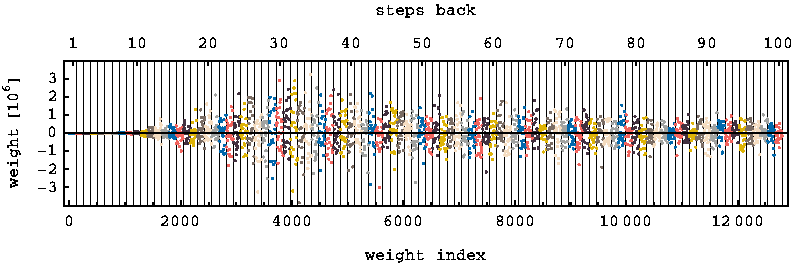
\includegraphics[width=0.99\linewidth]{pics/weight_plot}
	\caption{All weights $W_{i,s}$ attained through linear regression of the linear memory recalls $s \in [1,100]$ steps back. The system was a unidirectional ring with of $N_{real}=8$ and $N_{virtual}=16$ nodes. The total read-out dimension is $128$. For reconstruction of more recent inputs the inputs are small, but become enormous for inputs further in the past. This is the equivalent of "grasping at straws" as the system tries to extract information by multiplying microscopic fluctuations in the system state to linearily combine them to values between $[-1,1]$.}
	\label{fig:linearMemoryRecallWeights}
\end{figure}


\subsection{Reservoir computing tasks}

Typically reservoir computing tasks involve transformations on data sequences.

The reservoir computing performance of a given reservoir can be quantified by testing its predictions for certain tasks. The word "prediction" not necessarily means to predict the future value of something e.g. extend a timeseries into the future. Instead it often means the estimation of a value. A weather model which has been fed past temperature data can be tasked to "predict" the past humidity values. In machine learning the task is usually to predict a certain value or set of values from a set of inputs. Ideally the prediction can then be compared to the base truth and the difference between prediction and ground truth quantifies the error. The closer the prediction to the ground truth, the better the system performs a given task. 
It is important to note that usually these predictions are not of singular values, but give a vector of probabilities. A neural network used for image classification will output a vector with values e.g. it is quantifying the 'dog-ness', the 'tree-ness' or the 'car-ness' of an input image. The actual decision is made by choosing the entry with the highest probability. 
For predictions based on timeseries data the same applies. They are represented by continuous values that the system puts out. Even if the desired output is of discrete nature e.g. "yes" or "no" the system will usually output a real number. 

In general a sequence of inputs $u$ is drawn from a distribution. In this work only uniform distributions have been used. This sequence is used as input of a transformation which maps the sequence $u$ onto its target values $o$.


\subsection{Legendre polynomials as Nonlinear Transformations}

In order to investigate the nonlinear transformation capabilities one can use Legendre polynomials  (Fig. \ref{fig:legendreDegrees}) in order to transform inputs $\textbf{U}(t)$.	Legendre Polynomials have the useful property of being orthonormal to every other Legendre polynomial within an interval $\left[-1,1\right]$. This makes them highly useful for measuring linearily independent nonlinear (but also linear) transformation capacities. Legendre polynomials $L_{d}(x)$ for degrees $d \in \{1-5\}$ are shown in fig.\ref{fig:legendreDegrees}. Depending on the definition they are scaled so that $L_{d}(1)=1$. The Legendre polynomial $L_{1}(x)$ is of course simply the identity, which makes it possible to investigate the linear memory capacity also.

The idea of measuring nonlinear (as well as linear) transformation capacities through the means of Legendre polynomials is largely inspired from the publication \cite{DAM12}. Hence the terminology used in the latter shall be used here as well (where possible). 

	\begin{equation}
	f:U^{h}\rightarrow \mathbb{R}:u^{-h}\rightarrow f\left[ u^{-h}\right]
	\label{eq:legendre_f_U_equaiont}
	\end{equation}

All nonlinear transformations of an input sequence $\textbf{U}^{h}$ can be expressed as a linear combination of Legendre  polynomials with $h$ being the number of data points already fed into the system. With inputs in $\textbf{U}^{h}$ it is necessary to test all combinations. To elaborate: 
For a singular Legendre polynomial $L_{d_{1}}(\textbf{U}(t_1))$ with degree $d_1$ all values of $t_1$ have to be tested.
For the product of $2$ Legendre polynomials $L_{d_{1}}(\textbf{U}(t_1))$ and $L_{d_{2}}(\textbf{U}(t_2))$ with degrees $d_1$ and $d_2$ all combinations of $\textbf{U}(t_1)$ and $\textbf{U}(t_2)$ have to be calculated.
For the product of $3$ Legendre polynomials $L_{d_{1}}(\textbf{U}(-t_1))$, $L_{d_{2}}(\textbf{U}(-t_2))$ and $L_{d_{3}}(\textbf{U}(-t_3))$ all combinations of ${t_1,t_2,t_3}$ have to be tested.

So for the Product of $n$ Legendre polynomials there exist permutations ${\textbf{d}}={d_1,d_2,...d_n}$ of 






In order to investigate the different nonlinear transformation capabilities of a system it is necessary to iterate over all possible combinations of Products of Legendre polynomials  

\begin{figure}
	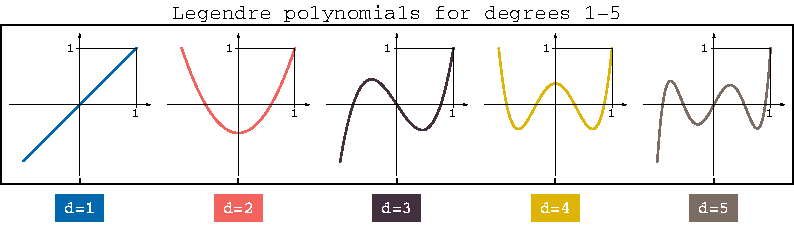
\includegraphics[width=0.99\linewidth]{pics/legendre_degrees}
	\caption{Legendre polynomials $L_{d}(x)$ for degrees $d \in \{1-5\}$ each shown for $x \in [-1,1]$ .}
	\label{fig:legendreDegrees}
\end{figure}

They are used in Neural networks as well blabla citecite findfind. 
\cite{VOELKER Legendre Memory Units: Continuous-TimeRepresentation in Recurrent Neural Networks}
%\begin{equation}


%\label{eq:legendrePolynomials}
%\end{equation}



\subsubsection{NARMA10 - the Nonlinear Autoregressive Moving Average Task}
\begin{equation}
A_{n+1} = 0.3 A_{n} + 0.05 A_{k}\left( \sum_{i=0}^{9} A_{k-9} \right) +1.5 u_{k-9} u_{k} + 0.1
\label{NARMA10equation}
\end{equation}

Lastly, the performance was investigated by measuring its capacity to compute the NARMA10 task. The Nonlinear Autoregressive Moving Average Task \cite{HER12} is used in many publications as a benchmark. The sequence is calculated using an average of its last $10$ steps while also being fed a product of a random sequence taken at two different positions. In order to perform well, systems need memory up to $10$ steps (hence the "10") into the past as well as nonlinear transformation capacities. Recently it has been shown that the task is not ideal as its difficulty depends non-trivially on the shape of the distribution used \cite{KUBOTA_Arxive}. \\
The NARMA10 sequence is created by the iterative formula given by \ref{NARMA10equation}. It is fed $2$ inputs from a sequence $u$ which is drawn from a uniform distribution $U(0,0.5)$ on interval $\left[0,0.5\right]$.



\begin{figure}[h]
	\centering
	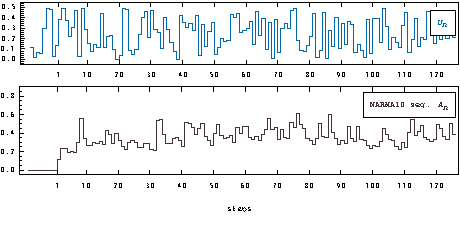
\includegraphics[width=13cm]{pics/narma_vis}
	\caption{Example for a uniformly drawn random sequence $U_n \in [0,0.5]$ that is used to create a Narma10 sequence $A_n$ with it. Here $A=0$ for $n<1$.}
	\label{fig:narma_vis}
\end{figure}
%here schöne plots mit narma.
	
	
	
	%order:
	%reservoir condition - fading memory etc.

\subsection{Stuart-Landau-Oscillator}
	The Stuart-Landau oscillator is a dynamical system often used to model basic class 1 lasers i.e. laser systems that do not exhibit pulsing or chaotic behavior (some refs). It can be written either as a single complex differential equation (\ref{eq:stuartlandauequation}) or a set of two equations written in polar coordinates (\ref{eq:stuartlandauequation_polar}). From the equation in polar coordinates easy to see that the equation has rotational symmetry as the radial differential equation does not change with the dynamical variable $\phi$. The Parameter $\lambda$ is often called the \emph{pump current} in accordance to its practical meaning.

\begin{equation}	
	\dot{z} = (\lambda +  i \omega + \gamma |z|^2 ) \; z
	\label{eq:stuartlandauequation}		
\end{equation}

\begin{equation}
	\begin{split}
	\dot{r} & = \lambda r + \operatorname{Re} (\gamma) \; r^{3} \\
	\dot{\phi} &= \omega + \operatorname{Im}(\gamma) \; r^{2} 
	\end{split}
	\label{eq:stuartlandauequation_polar}
\end{equation}

	For the radial dynamical variable the Stuart-Landau oscillator has two fixed points where the derivative $\dot{r}$ vanishes $r = 0$ and $r = \sqrt{-\lambda /\operatorname{Re}(\gamma)}$ whose stability depends on $\lambda$ and $\operatorname{Re}(\gamma)$. For $\operatorname{Re}(\gamma) < 0 $ (supercritical case).


\begin{figure}
	\centering
	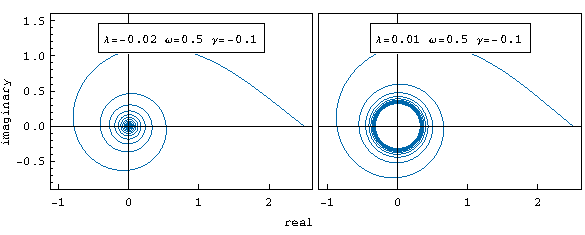
\includegraphics[width=0.99\linewidth]{pics/stuart_landau_complex_Focus_LC}
	\caption{$2$ very basic scenarios of the Stuart-Landau oscillator: Decay towards a single fixed point (off-state, left) or towards a stable oscillating state (limit cycle, right).}
	\label{fig:stuart_spiral}
	%nicht mehr
	%stuart_landau_basic.nb
\end{figure}


The limit cycle (LC) which is shown in fig \ref{fig:stuart_spiral} is depending on the ratio or $\lambda$ and $Re \left[\gamma \right]$.


As can be seen in (eq. \ref{eq:stuartlandauequation}), the equation has a linear and a nonlinear term regarding the absolute value of $z$.

\begin{equation}	
\dot{z} = (\lambda + G J(t) + i \omega + \gamma |z|^2 ) \; z + \kappa e^{i \phi} z(t-\tau)
\label{eq:stuartlandauequation_delayed_driven}		
\end{equation}

In this work we use a Stuart-Landau oscillator that has a varying bifurcation parameter $\hat{\lambda}(t)$ and a delayed feedback term $\kappa e^{i\phi}z(t-\tau)$. In our case $\hat{\lambda}(t)$ will always be an offset with only slight variations. We will therefore simply write  $\hat{\lambda}(t) = \lambda + G J(t)$ with $G \in \mathbb{R}$ being in the order of or exactly equal to $0.01$ (if not stated otherwise). The input signal $J(t)$ will be the actual variation that is used to feed data into the system (see Fig. \ref{fig:signal_mask_vis}). 

\begin{figure}
	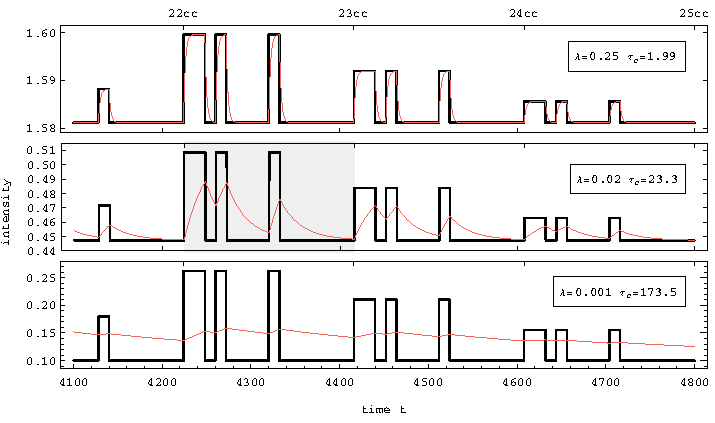
\includegraphics[width=15cm]{pics/different_lambda_values}
	\caption{Different values for $\lambda$ influence how fast the system's intensity \textcolor{myred}{\rule[2pt]{25pt}{2.5pt}} is responding to a given input signal. For a large value of $\lambda=0.25$ (top) the system's intensity almost instantaneously decays towards the expected limit cycle LC \rule[2pt]{25pt}{2.5pt}. The system is therefore determined exclusively by the current pump current. For intermediate values e.g. $\lambda=0.02$ (mid) the system's response is slower and can keep information longer. Very small values e.g. $\lambda=0.001$ (bottom) make the system respond too slow to react to a given input signal.}
	\label{fig:stuart_driven_landau_lambda_impact}
\end{figure}

\begin{figure}
	\centering
	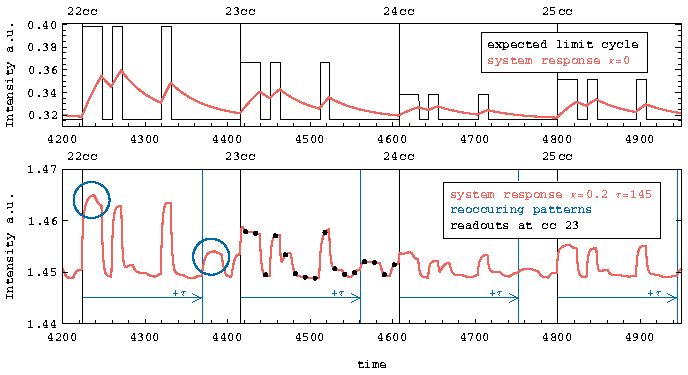
\includegraphics[width=15cm]{pics/driven_and_delayed}
	\caption{$|z|^{2}(t)$ of a driven Stuart-Landau oscillator with delayed feedback. Each clockcycle the system state is read out once per virtual node (red dots on the left). With delayed feedback patterns reappear after delay time $\tau$: the bump within the right blue rectangle is not caused by the input signal (above), but is an echo of the bump within the left blue rectangle. Without the delayed feedback ($\kappa=0$) the system response can be seen in the grey area in Fig.\ref{fig:stuart_driven_landau_lambda_impact}}
	\label{fig:driven_and_delayed}
\end{figure}

In Fig. \ref{fig:driven_and_delayed} a solution for $|z(t)|$ with and without delayed feedback is shown. Without it the intensity is exponentially decaying towards the new limit cycle (in black). With delayed feedback (bottom) previous inputs reappear: The little bump encased in the second blue circle is information that is fed back into the system. Usually the information isn't as visible or locally distinct, but a linear combination of all given readouts.



\subsection{Networks}

	\begin{figure}
		\centering
		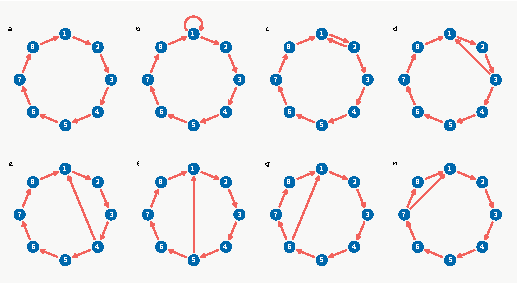
\includegraphics[width=12cm]{pics/graph_plot}
		\caption{example graph}
		\label{fig:example_graph}
	\end{figure}

Vertices blabla \
Edges blabla. \

	\subsubsection{circulant Matrix}
    A circulant matrix has the same entries its row vectors, but with its entries rotated one element to the right relative to the previous row.

    
\subsection{virtual Nodes and multiplexing}
	here: papers for explanation! 
	\cite{KUR18}
	
	\cite{STE20} // off-resonance = better! --> reason for choosing 17 * 12.
	
	By multiplexing the input signal one can create virtual nodes in a network. The analogy to a real network can be best understood if the input signal is masked with a binary mask containing only values of either $0$ or $1$. 
	
	Different Mask types: discrete values with constant interpolation: binary, uniform - easy to implement)
	continuous: any function or repeating noise-patterns. (more difficult, but )

	
	here add dependency of total linear memory on number of nodes and virtal nodes.

	
	\begin{figure}
		\centering
		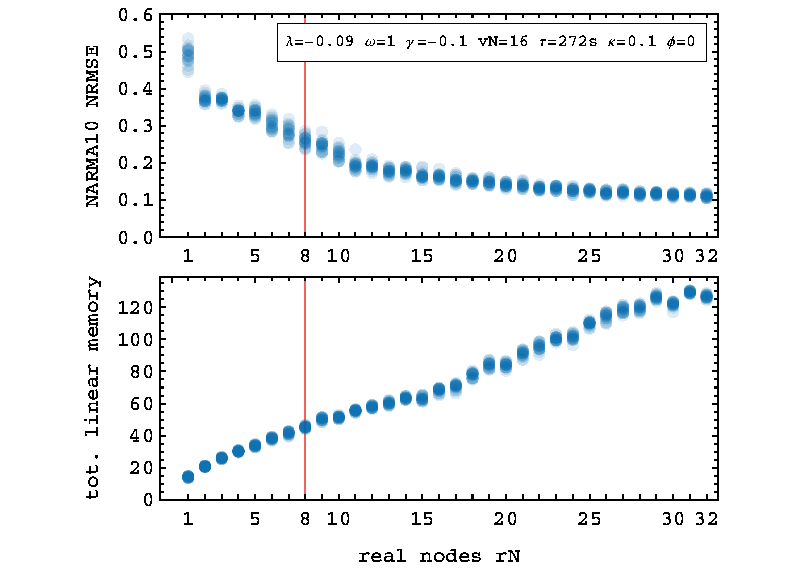
\includegraphics[width=0.9\linewidth]{pics/rNplot}
		\caption{changing rc performance for increasing number or real nodes $rN$ in unidirectianally coupled ring networks. (see some plot).}
		\label{fig:rN_1-32}
	\end{figure}

	\begin{figure}
		\centering
		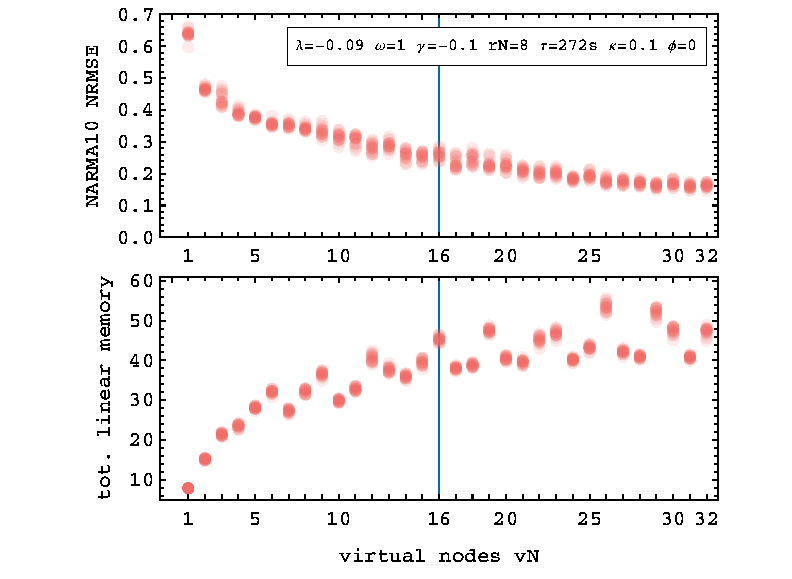
\includegraphics[width=15cm]{pics/vNplot}
		\caption{changing rc performance for increasing number or virtual nodes $rN$ in unidirectionally coupled ring networks. (see some plot).}
		\label{fig:vN_1-32}
	\end{figure}


\begin{figure}
	\centering
	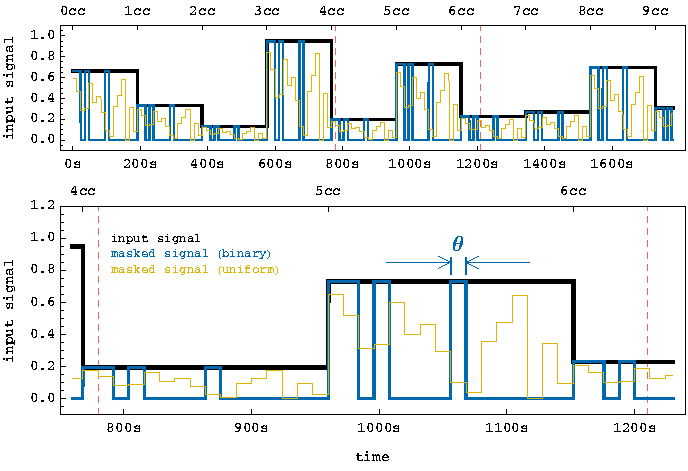
\includegraphics[width=15cm]{pics/signal_mask_vis}
	\caption{A timeseries of sampled data points \textcolor{myred}{\color{myred}$\sbullet[2]$}\,with its constant-interpolated signal between samples \rule[2pt]{25pt}{2.5pt}\, and the corresponding masked signals \textcolor{myblue}{\rule[2pt]{25pt}{2.5pt}} and \textcolor{myyellow}{\rule[2pt]{25pt}{2.5pt}}\,. The mask times (or lengths) are usually defined as $1$ clockcycle (cc, upper tick labels) and the time per virtual node called $\theta$. Here $\theta = 12$ and $1cc = 16 \theta = 272 $}
	\label{fig:signal_mask_vis}
	%feedInVis_stuartlandau.nb
\end{figure}



\subsection{Dynamics of rings of stuart landau oscillators}
	pony-states (von André)
	

	

% different stuart landau scenarios - hopf bifurcation